


\begin{frame}
\begin{center}
 
  Collective Annotation of WikiPedia Entities in Web Text 
  
  \bigskip
  
 \hyperref[thepaper]{ Sayali Kulkarni, Amit Singh, Ganesh Ramakrishnan, and Soumen Chakrabarti}
  \end{center}

\end{frame}

\begin{frame}
 \frametitle{Key Intuition : Topical Coherence}
 \begin{itemize}
  \item A document is usually about one topic \bigskip
  \item Disambiguating each entity using the local clues misses out on a major piece of information : Topic of a page \bigskip
  \item A page is usually has one topic, you can expect all the entities to be \emph{related} to the topic \emph{somehow} \bigskip
  \end{itemize}
  \textcolor{green}{Michael Jackson} : 30 Disambiguations 
  
 \textcolor{green}{John Paul} : 10 disambiguations 
 
 
 
  But if they are mentioned on the \textbf{same page}, the page is most likely about Christianity, A big hint towards disambiguating \textbf{both} of them
  
 
  \end{frame}
\begin{frame}{Topical Coherence}
  \begin{figure}[h]
 \centering
 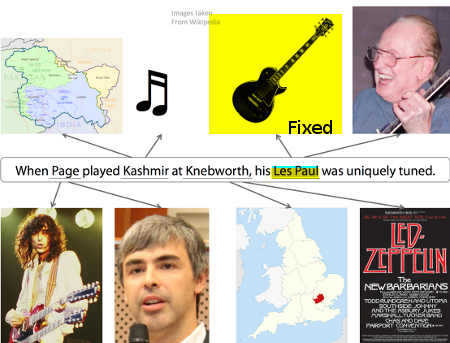
\includegraphics[bb=0 0 216 165]{./nedcollective.png}
 % nedcollective.png: 450x343 pixel, 150dpi, 7.62x5.81 cm, bb=0 0 216 165
\end{figure}

 \end{frame}

\begin{frame}{Challenges}
 \begin{itemize}
  \item Capturing local compatibility \medskip
  \begin{itemize}
   \item \textcolor{blue}{Create a scoring function to rank possible candidates}
  \end{itemize}

  \item Inculcating topical coherence in the overall objective \medskip

  \begin{itemize}
   \item \textcolor{blue}{Define Topical coherence}
  \end{itemize}

  \end{itemize}

\end{frame}

\begin{frame}
 \frametitle{Local compatibility}
 \begin{itemize}
  \item $s$ : Spot, an Entity to be disambiguated (Christian leader John Paul) \bigskip 
  \item $\gamma$ : An entity label value (\url{http://en.wikipedia.org/wiki/Po-pe_John_Paul_II})  \bigskip 
 \item $f_s(\gamma)$ : A feature function that creates a vector of features
 \end{itemize}

  
\end{frame}

\begin{frame}

\frametitle{Local compatibility : Feature design} 
\begin{itemize}
 \item 1. Take
\begin{itemize} 
 \item Text from the first descriptive paragraph of $\gamma$
  \item Text from the whole page for $\gamma$
  \item Anchor text within Wikipedia for $\gamma$.
  \item Anchor text and 5 tokens around $\gamma$ 
 \end{itemize}
 
 \item 2. Apply each of the following operation with one argument as Spot
    \begin{itemize}
      \item{Dot-product between word count vectors}
      \item{Cosine similarity in TFIDF vector space}
      \item{Jaccard similarity between word sets}
 \end{itemize} 
 \end{itemize}
 Total 12 Features (3 operations, 4 argument pairs) + Sense Probability Prior\footnote{Obtained by counting intra wiki links}
 
\end{frame}

\begin{frame}
 \frametitle{Compatibility Score}
 \begin{itemize}
 \item Local compatibility score between a spot $s$ and a candidate is given by $w^{T}f_s(\gamma)$ \medskip
 \item Thus, candidate is picked by $argmax_{\gamma\in\Gamma}w^{T}f_s(\gamma)$ \medskip
 \item $w$ is trained using an SVM like training objective 
 
 \begin{center} 
 Minimize $||w||^2 + C\Sigma_{s}\varepsilon_s$
 under the constraints
 $w^{T}f_s(\gamma) - w^{T}f_s(\gamma) \geq 1 - \varepsilon_s$ \end{center}
 \end{itemize}
 
 \end{frame}

\begin{frame}{Defining topic Relatedness}
  \begin{itemize}
   \item We need some notion of capturing the fact that 2 topics are related to each other \medskip
   \item Given
   \begin{itemize}
    \item $g(\gamma)$ : Set of wikipedia pages that link to $\gamma$
    \item $c :$ Total number of Wikipedia pages
    \item $r(\gamma, \gamma') :$ Relatedness of topics $\gamma$ and $\gamma'$
   \end{itemize}\bigskip

    
   \item Define $ r(\gamma, \gamma') = \frac{log|g(\gamma) \bigcap g(\gamma')| - log(max\{|g(\gamma)|, |(\gamma')|\})} {log c - log(min\{|g(\gamma)|, |(\gamma')|\})}$ 
  (The Milne and Witten Score)
  \end{itemize}

  
 \end{frame}

 
\begin{frame}
  \frametitle{The Dominant Topic Model}
  \begin{itemize}
   \item Need to define a collective score based on pairwise topical coherence of all $\gamma_s$ used for labeling. \medskip
   \item The pairwise topical coherence, $r(\gamma_s, \gamma_s')$ is as defined above.\medskip
   \item For a page, overall topical coherence : \begin{center}\medskip
                                                  $\Sigma_{s \neq s' \in S_0}r(\gamma_s, \gamma_s')$
                                                 \end{center}
   \item Can be written as clique potential as in case of node potential\medskip
      \begin{center}
	$exp(\Sigma_{s \neq s' \in S_0}r(\gamma_s, \gamma_s'))$
      \end{center}

  \end{itemize}

 \end{frame}

\begin{frame}
  \frametitle{The Optimization objective}
 \begin{center}
 \begin{empheq}[box={\mybluebox[5pt]}]{equation*}
  \frac{1}{\binom{|S_0|}{2}}\Sigma_{s \neq s' \in S_0}r(\gamma_s, \gamma_s') + \frac{1}{|S_0|}\Sigma_{s \in S_0}w^{T}f_s(\gamma)
 \end{empheq}
 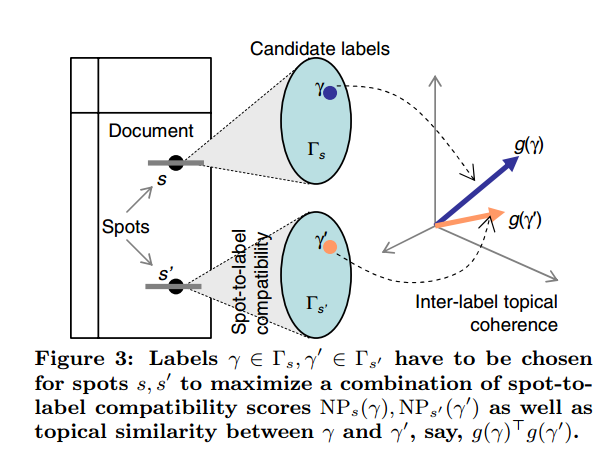
\includegraphics[height = 5 cm]{objective}\footnote{From \ref{thepaper}}
  \end{center}

 
 \end{frame}

\begin{frame}
  \frametitle{Solving the optimization objective}
  \begin{itemize}
   \item LP rounding approach\bigskip
   \item Hill climbing
   \begin{center}
    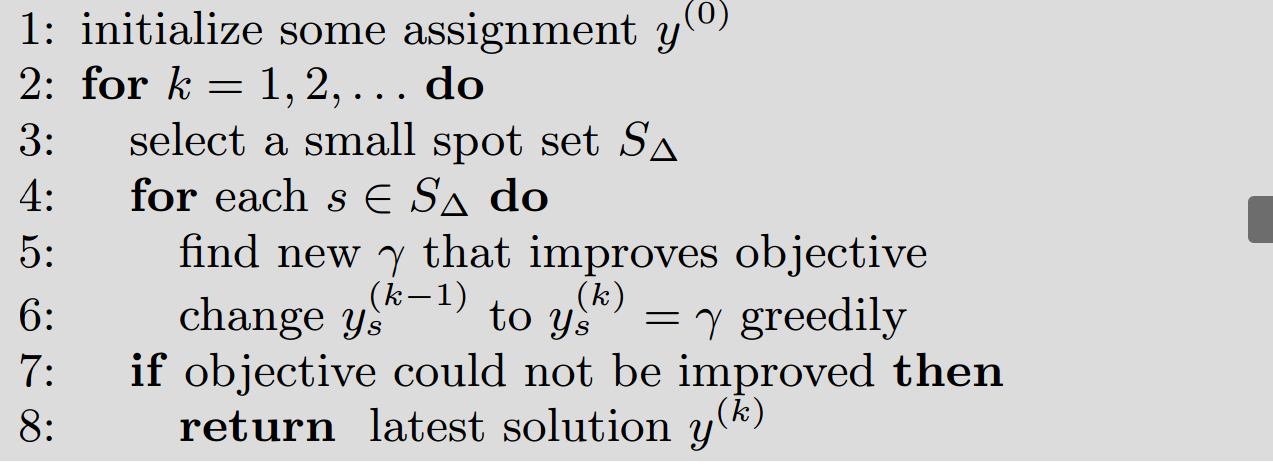
\includegraphics[height = 3cm]{hill}
   \end{center}

  \end{itemize}

 \end{frame}

\begin{frame}
  \frametitle{Experiments : Data preparation}
  \begin {itemize}
  \item August 2008 version of WikiPedia used, 5.15 million entity IDs. \medskip
  \item Filter out IDs composed of verbs, adverbs, conjunctions etc. \medskip
  \item Create a trie from IDs. \medskip
  \item Identify spots (\emph{NER}) by tokenizing the document and then matching spots with the trie. 
  \end{itemize}
  
 \end{frame}

\begin{frame}
  \frametitle{Experiments : Preparing Ground Truth Collection}
  \begin {itemize}
  \item Need data annotated with links to Wikipedia \medskip
  \item Done manually, pages obtained from popular links across various domains \medskip
  \item 19, 000 annotations marked, 40\% marked NA, 3800 distinct entities used \medskip
  \end{itemize}
 \begin{tabular}{| l | c | r |}
\hline
 Number of documents & 107 \\
Total number of spots & 17,200 \\

Spot per 100 tokens & 30 \\
Average ambiguity per Spot & 5.3\\
\hline
\end{tabular}
  
 \end{frame}

\begin{frame}
  \frametitle{Results : Only Local disambiguation}
  \begin{itemize}
  \item Local approach performs well
  \end{itemize}
  
  \begin{center}
  \begin{empheq}[box={\mybluebox[5pt]}]{equation*}
  \gamma_0 \leftarrow argmax_{\gamma\in\Gamma_s}  w^{T}f_s(\gamma)
  \end{empheq}
  \begin{empheq}[box={\mybluebox[5pt]}]{equation*}
  \text{if }  w^{T}f_s(\gamma_0) > \rho_{NA} \text{ then return }\gamma_0 \text{ else return NA}
  \end{empheq}
  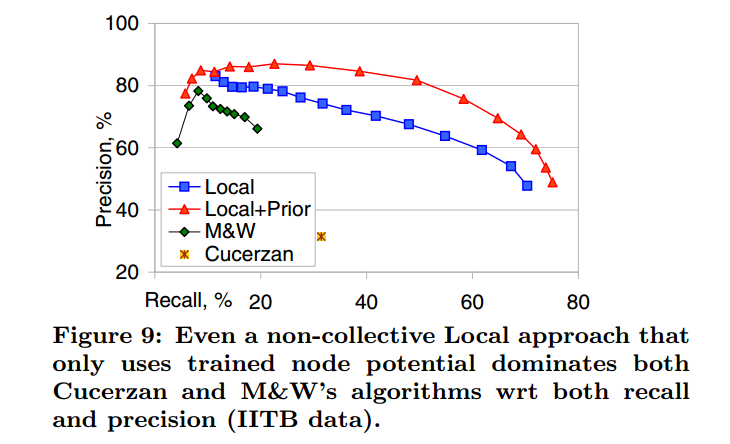
\includegraphics[height = 4 cm]{localperf}\footnote{from \ref{thepaper}}
  \end{center}

 \end{frame}

\begin{frame}
  \frametitle{LP vs Hill climbing approach}
  \begin{itemize}
   \item Hill climbing and LP are equivalent
  \end{itemize}

  \begin{center}
  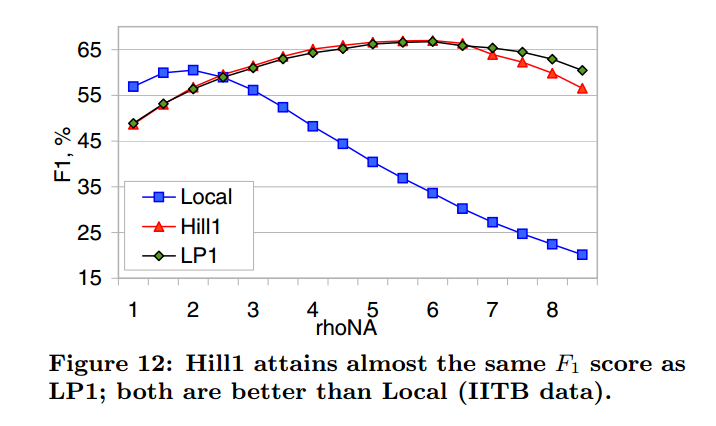
\includegraphics[height = 5 cm]{hillversuslp}\footnote{from \ref{thepaper}}
  \end{center}
 \end{frame}

 
\begin{frame}
  \frametitle{Recall precision for various approaches}
  \begin{itemize}
   \item Exploiting topical coherence improves precision by 9%
   \item Adding topic prior also helps
  \end{itemize}

  \begin{center}
  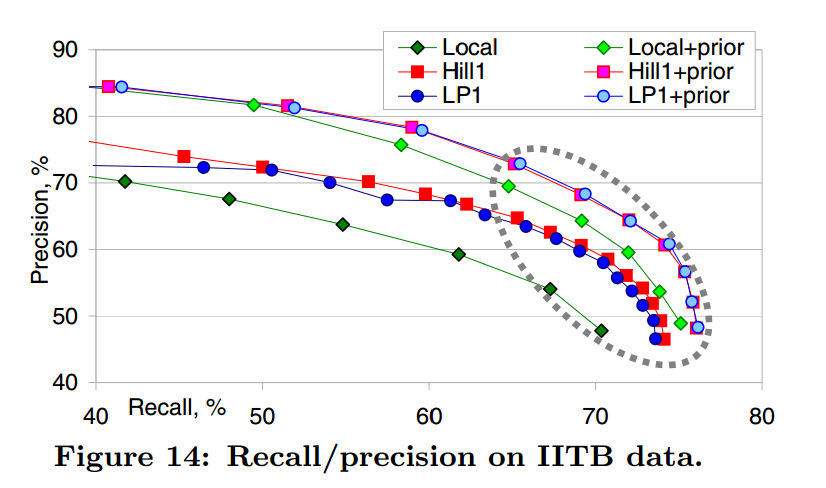
\includegraphics[height = 5 cm]{overall}\footnote{from \ref{thepaper}}
  \end{center}
 \end{frame}